\documentclass[15pt, a4paper]{article}
\usepackage[T1]{fontenc}
\usepackage[polish]{babel}
\usepackage[utf8]{inputenc}
\usepackage{tikz}
\usepackage{adjustbox}
\usepackage{longtable}
\usepackage{graphicx}
\usepackage{amsfonts}
\usepackage{algpseudocode}
\usepackage{algorithm}
\usepackage{amsmath}
\title{Obliczenia naukowe}
\author{Felix Zieliński 272336}
\date{Lista 3}
\begin{document}
\maketitle

nwm jakies wnioski, czym sie roznia te metody czy cos, nazwy returnowanych w kodzie
metoda DOJEBANEGO Eulera (tak naprawde to nie ale bardzo chcialem to napisac)
iteracje w 6.2 dla f1???
moze wiecej testow bo nwm w sumie cyz nie za malo + jakies jak sie wysrywa + moze dla innych funkcji
wnioski koncowe idk

\vspace{0.5cm}

\noindent\hrulefill

\vspace{0.5cm}

% zadanie 1

\noindent\textbf{Zadanie 1.} Funkcja rozwiązująca równanie \( f(x) = 0 \) metodą bisekcji.\\\\
\noindent Metoda bisekcji to inaczej metoda równego podziału lub metoda połowienia. 
Korzysta ona z faktu, że funkcja ciągła w przedziale \( [a, b] \), która zmienia w nim swój znak (a więc \( f(a) * f(b) < 0 \)), musi mieć miejsce zerowe w \( (a, b) \).\\\\
\noindent Jeżeli \( f(a) * f(b) < 0 \), to wiem, że gdzieś na przedziale jest miejsce zerowe. Obliczam więc takie \(c\), że \( c = 1/2 * (a + b) \) (połowa przedziału) i sprawdzam z tego samego warunku, czy jest tam miejsce zerowe. Jeżeli tak, to podstawiam \( b = c \), a w przeciwmym razie \( a = c \).\\\\
\noindent Powtarzam to, dopóki nie znajdę zera (bo \( f(a) * f(c) = 0 \) lub \(f(b) * f(c) = 0 \)). \\\\
\noindent W ten sposób jednak, otrzymam tylko jedno miejsce zerowe, nawet jeśli jest ich więcej na tym odcinku.\\\\ 
\noindent Innym warunkiem zakończenia jest warunek \(|f(c)| < \epsilon \) lub \(|b - a| < \delta \). Te stałe są podane przy wywołaniu funkcji i decydują o dokładności wyniku, bowiem dla typu zmennoprzecinkowego \(Float64\) mogą oczywiście nastąpić błędy przybliżeń. \( \epsilon \) jest wartością błędu przybliżenia, a \(\delta\) - pożądaną bliskością otrzymanej wartości iloczynu do zera. 

\pagebreak

\begin{algorithm}
\caption{Metoda bisekcji}
\label{alg:metoda_bisekcji}
\begin{algorithmic}[1]
\Function{mbisekcji}{$f$, $a$, $b$, $\delta$, $\epsilon$}
    \State $a\_val \gets f(a)$
    \State $b\_val \gets f(b)$
    \State $interval \gets b - a$
    \State $iterations \gets 0$
    \State $c \gets 0$
    \State $middle\_val \gets 0$\\

    \If{$\text{sign}(a\_val) = \text{sign}(b\_val)$}
        \State \Return \text{error}
    \EndIf\\

    \While{$interval > \epsilon$}
        \State $iterations \gets iterations + 1$
        \State $interval \gets interval / 2$
        \State $c \gets a + interval$
        \State $middle\_val \gets f(c)$\\

        \If{$|middle\_val| < \epsilon$ \textbf{or} $|interval| < \delta$}
            \State \Return $(c, middle\_val, iterations, 0)$
        \EndIf\\

        \If{$\text{sign}(middle\_val) = \text{sign}(a\_val)$}
            \State $a \gets c$
            \State $a\_val \gets middle\_val$
        \Else
            \State $b \gets c$
            \State $b\_val \gets middle\_val$
        \EndIf
    \EndWhile\\

    \State \Return $(c, middle\_val, iterations, 0)$\\
\EndFunction
\end{algorithmic}
\end{algorithm}



\vspace{0.5cm}

\noindent\hrulefill

\vspace{0.5cm}

% zadanie 2 

\noindent\textbf{Zadanie 2.} Funkcja rozwiązująca równanie \( f(x) = 0 \) metodą Newtona.\\\\
\noindent To inaczej metoda stycznych. Działa ona dla funkcji, która w przedziale \([a, b]\) musi znajdować się dokładnie jeden jej pierwiastek,  \(f(a) * f(x) < 0 \) oraz jej pierwsza i druga pochodna mają stały znak w przedziale \( [a, b] \).\\\\
\noindent Liczę punkty przecięcia stycznych do funkcji z osią \( OX \), zaczynając od prostej stycznej w \( f(x_0) \). Współrzędnia \(x\), w której styczna przecina oś \(OX\), jest przybliżeniem pierwiastka funkcji. Szukam dalej przybliżeń, aż w końcu któreś spełni dane założenia. 


\begin{algorithm}
\caption{Metoda stycznych}
\label{alg:metoda_stycznych}
\begin{algorithmic}[1]
\Function{mstycznych}{$f$, $pf$, $x_0$, $\delta$, $\epsilon$, $maxit$}
    \State $val \gets f(x_0)$\\

    \If{$|val| < \epsilon$}
        \State \Return $(x_0, val, 0, 0)$
    \EndIf\\

    \If{$|pf(x_0)| < \epsilon$}
        \State \Return \text{error}
    \EndIf\\

    \State $x \gets 0$\\

    \For{$i \gets 1$ \textbf{to} $maxit$}
        \State $x \gets x_0 - \frac{val}{pf(x_0)}$
        \State $val \gets f(x)$\\

        \If{$|val| < \epsilon$ \textbf{or} $|x - x_0| < \delta$}
            \State \Return $(x, val, i, 0)$
        \EndIf\\

        \State $x_0 \gets x$
    \EndFor\\

    \State \Return \text{error}\\
\EndFunction
\end{algorithmic}
\end{algorithm}

\vspace{0.5cm}

\noindent\hrulefill

\vspace{0.5cm}

% zadanie 3

\noindent\textbf{Zadanie 3.} Funkcja rozwiązująca równanie \( f(x) = 0 \) metodą siecznych.\\\\
\noindent To inaczej metoda cięciw lub Eulera. Działa ona dla funkcji, która jest dwukrotnie rózniczkowalna na przedziale \([a, b]\) oraz pierwiastek szukany musi być nieparzystej krotności. \\\\
\noindent W tej metodzie używa się ilorazu różnicowego zamiast pochodnej \(f'(x_n) \approx \frac{f(x_n) - f(x_{n-1})}{x_n - x_{n-1}}\). Sama metoda siecznych opisana jest wzorem \(x_{n+1} = x_n - f(x_n) \frac{x_n - x_{n-1}}{f(x_n) - f(x_{n-1})}\) dla dodatnich n.\\\\
\noindent Wyznaczam miejsca przecięć siecznych funkcji z osią \(OX\), rozpoczynając od siecznej mającej swój początek w punkcie \((x_0, f(x_0))\) oraz koniec w \((x_1, f(x_1))\). Sieczna ta przecina oś \(OX\) w \(x_2\), którego używam do wyznaczenia kolejnej siecznej i jej przecięcia z osią. \\\\
\noindent Szukanie przybliżenia pierwiastka kończy się, gdy przybliżenie zera będzie odpowiednio małe (zgodne z podanym do funkcji), bądź gdy różnica między kolejnymi przybliżeniami będzie wystarczająco mała (zgodna z podanym do funkcji).


\begin{algorithm}
\caption{Metoda siecznych}
\label{alg:secant_method}
\begin{algorithmic}[1]
\Function{msiecznych}{$f$, $x_0$, $x_1$, $\delta$, $\epsilon$, $maxit$}
    \State $f_a \gets f(x_0)$
    \State $f_b \gets f(x_1)$\\

    \For{$i \gets 1$ \textbf{to} $maxit$}
        \If{$|f_a| > |f_b|$}
            \State $(f_a, f_b) \gets (f_b, f_a)$
            \State $(x_0, x_1) \gets (x_1, x_0)$
        \EndIf\\

        \State $s \gets \frac{x_1 - x_0}{f_b - f_a}$
        \State $x_1 \gets x_0$
        \State $f_b \gets f_a$
        \State $x_0 \gets x_0 - (f_a \cdot s)$
        \State $f_a \gets f(x_0)$\\

        \If{$|x_1 - x_0| < \delta$ \textbf{or} $|f_a| < \epsilon$}
            \State \Return $(x_0, f_a, i, 0)$
        \EndIf
    \EndFor\\ 

    \State \Return \text{error}\\
\EndFunction
\end{algorithmic}
\end{algorithm}

\vspace{0.5cm}

\noindent\hrulefill

\vspace{0.5cm}

%zadanie 4

\noindent\textbf{Zadanie 4} W tym zadaniu należało wyznaczyć pierwiastki funkcji \(\sin x - \left(\frac{1}{2}x\right)^2\) przy użyciu metod zaprogramowanych w poprzednich zadaniach.\\\\
\noindent Wyniki dla poszczególnych metod przedstawia poniższa tabela:

\begin{table}[ht]
\begin{adjustbox}{max width=\textwidth}
\begin{tabular}{|c|c|c|c|c|}
    \hline
    \textbf{Metoda} & \textbf{x0} & \textbf{f(x0)} & \textbf{Iteracje} & \textbf{Czy błąd} \\
    \hline
    Medota bisekcji & 1.9337539672851562 & -2.7027680138402843e-7 & 16 & false \\
    \hline
    Metoda Newtona & 1.933753779789742 & -2.2423316314856834e-8 & 4 & 0 \\
    \hline
    Metoda siecznych & 1.933753644474301 & 1.564525129449379e-7 & 4 & false \\
    \hline
\end{tabular}
\end{adjustbox}
\end{table}


\noindent Metoda bisekcji potrzebowała najwiecej iteracji, bo aż 16, podczas gdy pozostałe metody potrzebowały ich tylko 4. Metoda Newtora oraz siecznych mają mniejszą złożoność. Każda z metod obliczyła wartość pierwiastka z podobną dokładnością.

\vspace{0.5cm}

\noindent\hrulefill

\vspace{0.5cm}

%zadanie 5

\noindent\textbf{Zadanie 5.} Wyznaczenie wartości zmiennej x, dla której wykresy \( y = 3x \) oraz \( y = e^x \) się przecinają.\\\\
\noindent W zadaniu tym posłużę się faktem, że skoro \(3x = e^x \), to \(3x - e^x = 0 \). Dla takiej też funkcji będę wyszukiwał miejsce zerowe. Aby móc jednak wyznaczyć je tą metodą, muszę poznać, jak przebiega jej zmienność w celu odpowiedniego dobrania punktów a oraz b, dlatego też narysowałem wykresy obu funkcji:\\

\begin{figure}[h]
    \centering
    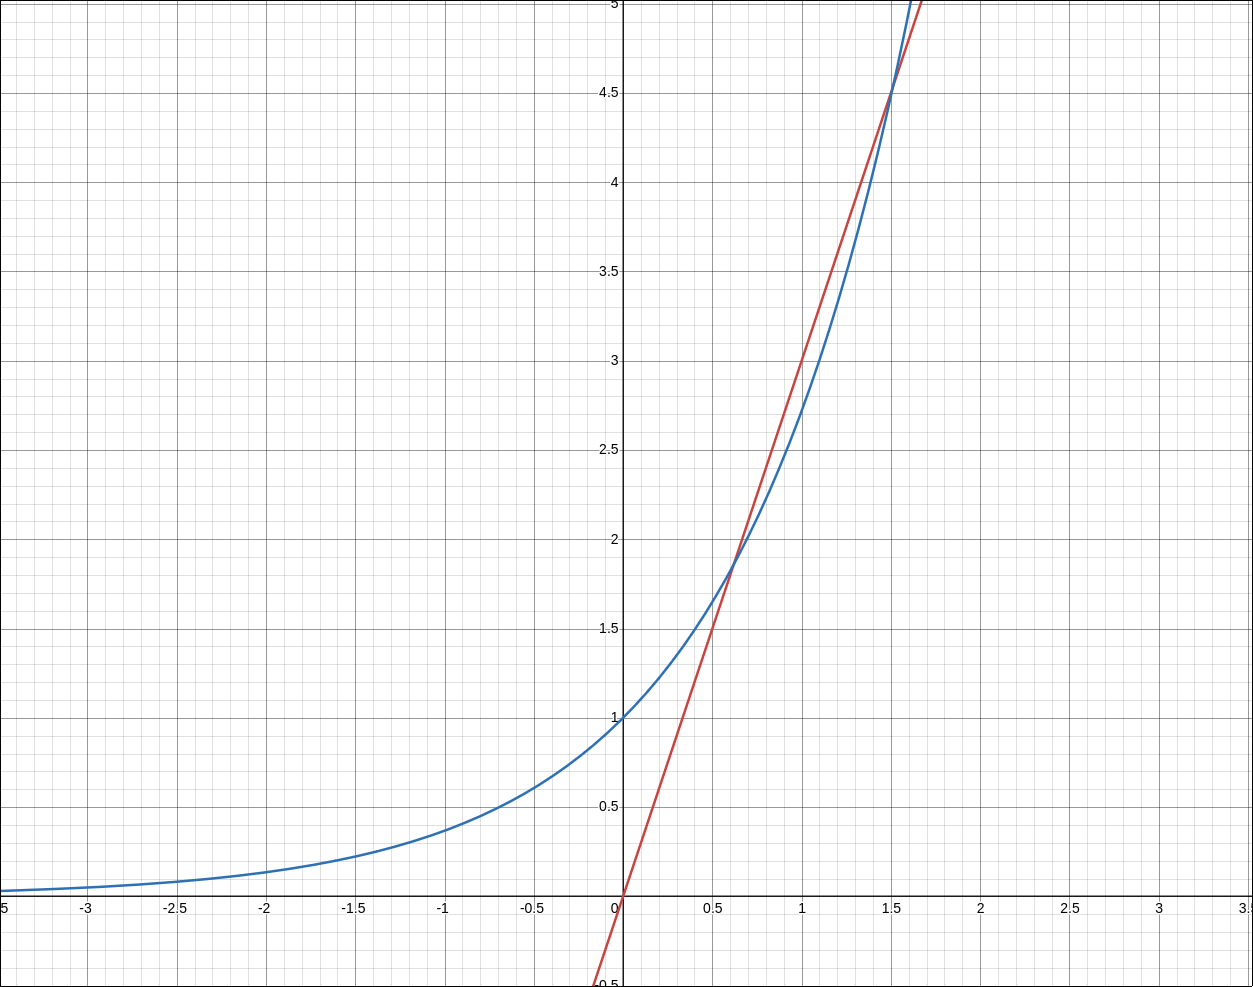
\includegraphics[width=0.5\textwidth]{img/wykreszad5.png}
\end{figure}

\noindent Wyniki przedstawia poniższa tabela

\begin{table}[ht]
\begin{adjustbox}{max width=\textwidth}
\begin{tabular}{|c|c|c|c|c|}
    \hline
    \textbf{Przedział} & \textbf{x0} & \textbf{f(x0)} & \textbf{Iteracje} & \textbf{Czy błąd} \\
    \hline
    [0.0, 1.0] & 0.619140625 & 9.066320343276146e-5 & 9 & false \\
    \hline
    [1.0, 2.0] & 1.5120849609375 & 7.618578602741621e-5 & 13 & false \\
    \hline
    [0.0, 2.0] & NaN & NaN & 0 & true \\
    \hline
\end{tabular}
\end{adjustbox}
\end{table}

\noindent Jak widać, aby dobrze wyznaczyć punkty przecięcia funkcji (miejsca zerowe) przy użyciu metody bisekcji, powinno się posiadać informacje o przebiegu zmienności funkcji. W przypadku złebo dobrania przedziału, nie będzie można uzyskać prawidłowego wyniku (jak dla [0.0, 2.0], gdzie na jego krańcach funkcja nie zmienia znaku). W tym zadaniu, prawdopodobnie lepiej byłoby zastosować metodę Newtona bądź siecznych, gdyż nie wymagają one dokładnej znajomości jej przebiegu.

%TODO: CZY NEI PISZE GLUPOT

\vspace{0.5cm}

\noindent\hrulefill

\vspace{0.5cm}

%zadanie 6

\noindent\textbf{Zadanie 6.} Znalezienie miejsc zerowych funkcji \( f_1(x) = e^{1-x} - 1 \) oraz \(f_2(x) = xe^{-x}\) za pomocą trzech powyższych metod.\\\\
\noindent W celu wyznaczenia przedziału, zwizualizowałem wykresy tych funkcji: \\

\begin{figure}[h]
    \centering
    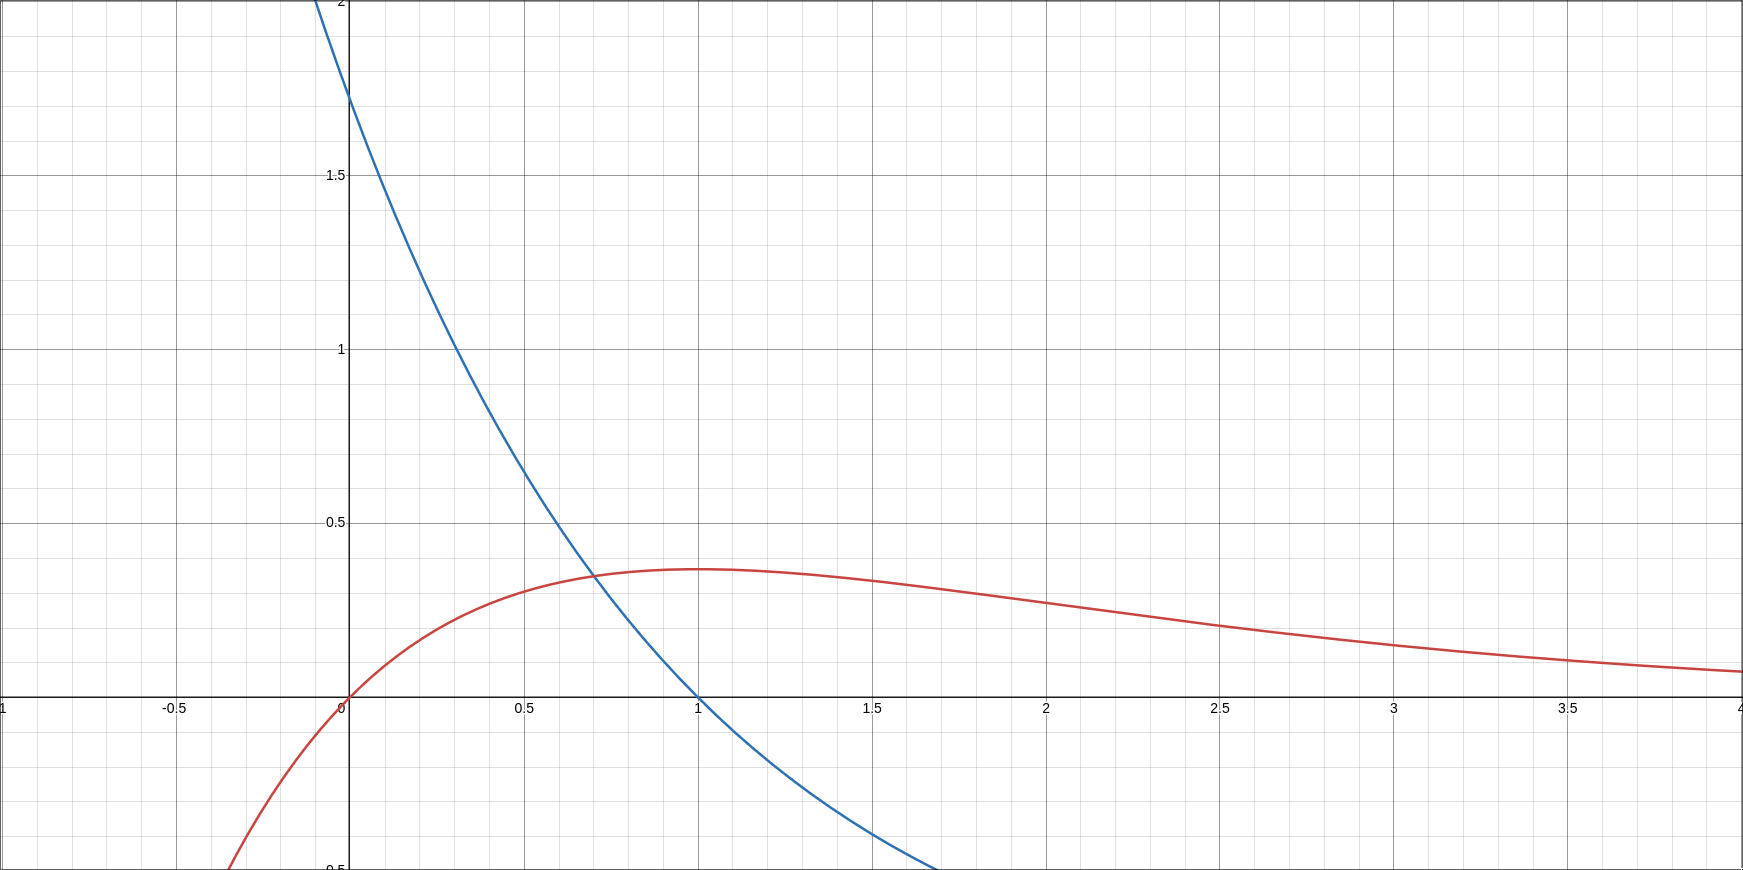
\includegraphics[width=0.5\textwidth]{img/wykreszad6.png}
\end{figure}

\noindent Z powyższego wykresu można odczytać, że funkcja \(f_1 \) ma miejce zerowe w 1, a \(f_2\) w 0.\\ 

\noindent Najpierw sprawdziłem, jakie wyniki otrzymam metodą bisekcji. Dobrałem w tym celu rózne przedziały.\\

\noindent Wyniki dla f1:
\begin{table}[ht]
\begin{adjustbox}{max width=\textwidth}
\begin{tabular}{|c|c|c|c|c|}
    \hline
    \textbf{Przedział} & \textbf{x0} & \textbf{f(x0)} & \textbf{Iteracje} & \textbf{Czy błąd} \\
    \hline
    [0.0, 1.0] & 0.9999923706054688 & 7.629423635080457e-6 & 17 & false \\
    \hline
    [-1.0, 1.0] & 0.9999923706054688 & 7.629423635080457e-6 & 18 & false \\
    \hline
    [-3.0, 3.0] & 1.0000076293945312 & -7.6293654275305656e-6 & 18 & false \\
    \hline
    [-0.0, 2.0] & 1.0 & 0.0 & 1 & false \\
    \hline
\end{tabular}
\end{adjustbox}
\end{table}

\noindent Wyniki dla f2:
\begin{table}[ht]
\begin{adjustbox}{max width=\textwidth}
\begin{tabular}{|c|c|c|c|c|}
    \hline
    \textbf{Przedział} & \textbf{x0} & \textbf{f(x0)} & \textbf{Iteracje} & \textbf{Czy błąd} \\
    \hline
    [0.0, 1.0] & 7.62939453125e-6 & 7.62933632381113e-6 & 17 & false \\
    \hline
    [-1.0, 1.0] & 0.0 & 0.0 & 1 & false \\
    \hline
    [-0.4, 0.5] & -1.5258789062623358e-6 & -1.5258812345705489e-6 & 16 & false \\
    \hline
    [-0.5, 0.5] & 0.0 & 0.0 & 1 & false \\
    \hline
\end{tabular}
\end{adjustbox}
\end{table}

\noindent Można zauważyć, że dobrany przedział wpływa na dokładność wyniku, oraz na liczbę potrzebnych iteracji tej metody.\\\\

\pagebreak

\noindent Dla metody Newtona przyjąłem \(maxit = 100 \).\\

\noindent Wyniki dla f1:
\begin{table}[ht]
\begin{adjustbox}{max width=\textwidth}
\begin{tabular}{|c|c|c|c|c|}
    \hline
    \textbf{Początkowe x0} & \textbf{x0} & \textbf{f(x0)} & \textbf{Iteracje} & \textbf{Czy błąd} \\
    \hline
    0.0 & 0.9999984358892101 & 1.5641120130194253e-6 & 4 & 0 \\
    \hline
    0.5 & 0.9999999998878352 & 1.1216494399945987e-10 & 4 & 0 \\
    \hline
    0.9999 & 0.9999999950001667 & 4.999833436158951e-9 & 1 & 0 \\
    \hline
    1.0 & 1.0 & 0.0 & 0 & 0 \\
    \hline
    2.0 & 0.9999999810061002 & 1.8993900008368314e-8 & 5 & 0 \\
    \hline
    10.0 & NaN & NaN & - & 1 \\
    \hline
\end{tabular}
\end{adjustbox}
\end{table}

\noindent Wyniki dla f2:
\begin{table}[ht]
\begin{adjustbox}{max width=\textwidth}
\begin{tabular}{|c|c|c|c|c|}
    \hline
    \textbf{Początkowe x0} & \textbf{x0} & \textbf{f(x0)} & \textbf{Iteracje} & \textbf{Czy błąd} \\
    \hline
    -1.0 & -3.0642493416461764e-7 & -3.0642502806087233e-7 & 5 & 0 \\
    \hline
    -1.0e-5 & -9.99990000100624e-11 & -9.999900002006219e-11 & 1 & 0 \\
    \hline
    0.0 & 0.0 & 0.0 & 0 & 0 \\
    \hline
    0.5 & -3.0642493416461764e-7 & -3.0642502806087233e-7 & 5 & 0 \\
    \hline
    1.0 & NaN & NaN & - & 2 \\
    \hline
    10.0 & 14.380524159896261 & 8.173205649825554e-6 & 4 & 0 \\
    \hline
\end{tabular}
\end{adjustbox}
\end{table}

\noindent W tej metodzie również odpowiednio dobrana wartość początkowa \( x_0 \) pozwala na ograniczenie liczby iteracji, oraz w ogóle na poprawność wyniku.\\ 
W pzypadku wybrania \(x_0 = 1\) dla \(f2\) nie udało się uzyskać wyniku, gdyż wartość pochodnej w tym punkcie wynosi 0, a wieć styczna jest równoległa do osi \(OX\), co uniemożliwia wyznaczenie kolejnego punktu przecięcia, i tym samym - poprawnego obliczenia wyniku. 

%TODO: f1???????? dla duzyc?????

\noindent Metoda Newtona dla \(f2\), w przypadku dobrania nieodpowiedniej wartości początkowej (np \(x_0 > 1\)) szuka miejsca zerowego zmierzając w kierunku zbiegania funkcji do 0 (bowiem, jak widać na wykresie, funkcja ta jest zbieżna do 0 w nieskończoności), co skutkuje nieprawidłowym wynikiem. 

%TODO  czy to prawda w ogole?

\pagebreak

\noindent Dla metody siecznych przyjąłem taką samą wartość maxit.

\noindent Wyniki dla f1:
\begin{table}[ht]
\begin{adjustbox}{max width=\textwidth}
\begin{tabular}{|c|c|c|c|c|c|}
    \hline
    \textbf{Początkowe x0} & \textbf{Początkowe x1} & \textbf{x} & \textbf{f(x)} & \textbf{Iteracje} & \textbf{Czy błąd} \\
    \hline
    0.0 & 0.5 & 0.9999998133327657 & 1.8666725165594755e-7 & 5 & false \\
    \hline
    0.5 & 0.6 & 0.9999946034580037 & 5.396556557624166e-6 & 4 & false \\
    \hline
    0.9999 & 0.999999 & 0.9999999999500008 & 4.9999338003203775e-11 & 1 & false \\
    \hline
    1.0 & 1.05 & 1.0 & 0.0 & 1 & false \\
    \hline
    2.0 & 1.5 & 1.0000034269838276 & -3.4269779555229363e-6 & 5 & false \\
    \hline
    10.0 & 14.0 & 10.0 & -0.9998765901959134 & 2 & false \\
    \hline
\end{tabular}
\end{adjustbox}
\end{table}

\noindent Wyniki dla f2:
\begin{table}[ht]
\begin{adjustbox}{max width=\textwidth}
\begin{tabular}{|c|c|c|c|c|c|}
    \hline
    \textbf{Początkowe x0} & \textbf{Początkowe x1} & \textbf{x} & \textbf{f(x)} & \textbf{Iteracje} & \textbf{Czy błąd} \\
    \hline
    -1.0 & -0.5 & -1.2229958402039555e-7 & -1.2229959897758473e-7 & 6 & false \\
    \hline
    -1.0e-5 & -1.0e-7 & -9.999949500039373e-13 & -9.999949500049373e-13 & 1 & false \\
    \hline
    0.0 & 0.5 & 0.0 & 0.0 & 1 & false \\
    \hline
    0.5 & 0.3 & -1.1876245840531925e-7 & -1.187624725098416e-7 & 6 & false \\
    \hline
    1.0 & 0.0 & 0.0 & 0.0 & 1 & false \\
    \hline
    10.0 & 15.0 & 15.05105056651027 & 4.375005536508203e-6 & 1 & false \\
    \hline
\end{tabular}
\end{adjustbox}
\end{table}

\noindent Wybór odpowiednich wartości początkowych również i przy tej metodzie ma wpływ na ilość iteracji. Niepoprawne dobranie ich dla funkcji \(f2\) również i tutaj powoduje pojawienie się skrajnie niepoprawnych wyników przez jej zbieżność do 0 w nieskończoności.\\ 

%TODOL ZNOWU, CZY NIE PISZE GLUPOT

\noindent Dla metody bisekcji, przydatna jest znajomość przebiegu funkcji, aby odpowiednio dobrać przedział. Najlepsze wyniki są wtedy, gdy przedział jest odpowiednio wąski, a miejsce zerowe znajduje się na jego środku. \\\\
Dla metody Newtona oraz siecznych wpływ wartości początkowych \(x_0\) oraz \(x_1\) jest znaczny. Im są one lepszymi przybliżeniami faktycznego miejsca zerowego, tym dokładniejszy będzie wynik.\\\\



\end{document}
